\chapter{JIAC Node Plugin}
\label{sec:user_jiac-node}

Not actually a part of the VSDT, but closely related, is the so-called \emph{JIAC
Node Plugin}, which will be the topic of this chapter.

The central part of the JIAC Node Plugin is -- as the name suggests -- a JIAC
agent node~\cite{lutzenberger2013jiacShort,luetze2015jiacChapter} running 
\emph{inside} of an Eclipse plug-in, which can be used as a platform for several
applications, integrating features provided by JIAC agents (both running on the
node itself \emph{and} on other nodes in the network) with into the Eclipse
environment. In the following, we will introduce some especially graphic
applications for the JIAC Node Plugin.

The JIAC node can either use \emph{multicast} or a \emph{gateway} for communication,
and depending on which is used, different external agents and nodes will be found.
This setting can be changed in the preferences (\emph{Window $\rightarrow$
Preferences $\rightarrow$ JIAC Node Plugin}).

For more about JIAC itself, please refer to the JIAC manual~\cite{jiacManual}.


%%%%%%%%%%%%%%%%%%%%%%%%%%%%%%%%%%%%%%%%%%%%%%%%%%%%%%%%%%%%%%%%%%%%%%%%%%%%%%%%
%%  JIAC Multicast-Chat View                                                  %%
%%%%%%%%%%%%%%%%%%%%%%%%%%%%%%%%%%%%%%%%%%%%%%%%%%%%%%%%%%%%%%%%%%%%%%%%%%%%%%%%

\section{JIAC Multicast-Chat View}

The \emph{JIAC Multicast-Chat} was the first application developed for the JIAC
Node Plugin.  It is, in essence, a simple Chat application running inside of
Eclipse, making use of JIAC's communication infrastructure.  While not being overly
useful, given the abundance of existing chat programs, the ease of integrating a
chat view into Eclipse using the JIAC Node Plugin is compelling.  Therefore, the
Multicast-Chat can also be seen as an elaborate tutorial for developing other
JIAC-based Eclipse plug-ins.

\begin{figure}[ht]
	\centering
	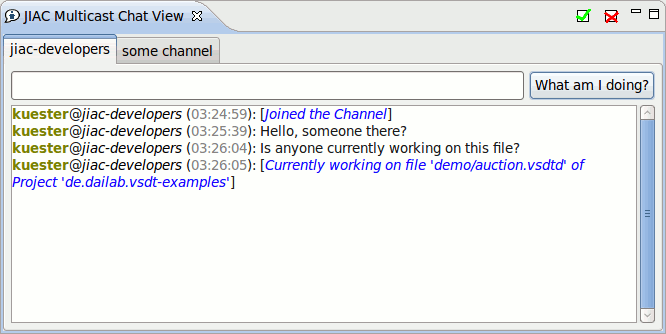
\includegraphics[width=.5\textwidth]{figures/features/multicast-chat.png}
	\caption{The JIAC Multicast-Chat View.}
	\label{fig:chatView}
\end{figure}

The Multicast-Chat View, as seen in Figure~\ref{fig:chatView}, allows the user to
subscribe to one or more chat channels, each one corresponding to a multicast
group channel in JIAC.  The user can then send messages to fellow developers being
subscribed to the same channel.  Since the multicast-chat is aimed especially at
developers working in their Eclipse IDEs at the same time, a special feature of
the Multicast-Chat is to broadcast which file of code one is currently working
on, possibly alleviating problems due to conflicting changes on that file.


%%%%%%%%%%%%%%%%%%%%%%%%%%%%%%%%%%%%%%%%%%%%%%%%%%%%%%%%%%%%%%%%%%%%%%%%%%%%%%%%
%%  JIAC Service-Deployment View                                              %%
%%%%%%%%%%%%%%%%%%%%%%%%%%%%%%%%%%%%%%%%%%%%%%%%%%%%%%%%%%%%%%%%%%%%%%%%%%%%%%%%

\section{JIAC Service Deployment View}

Another, much more useful view is the \emph{JIAC Service Deployment View}, shown
in Figure~\ref{fig:deployView}.  This view uses JIAC's service-discovery and
-invocation mechanisms to provide a number of features to the user:

\begin{itemize}
	\item \emph{Look up} services currently being provided by other JIAC agents in
	the network, displaying them in a tree view, grouped by agent and agent node,

	\item \emph{import} those services (both actions provided by JIAC agent beans
	and JADL services) as Service descriptions into the current VSDT diagram, so
	they can be reused and orchestrated to new services,

	\item \emph{deploy} new services composed in the VSDT\footnote{VSDT Process
	Diagrams will be exported to JADL services prior to being deployed on the
	JADL interpreter.} or in the JADL editor to some JADL interpreter agent
	currently running on some node,

	\item \emph{invoke} services and actions being provided by some JIAC agent on
	the network, including the ones just deployed, and

	\item \emph{undeploy} services.
\end{itemize}

\begin{figure}[ht]
	\centering
	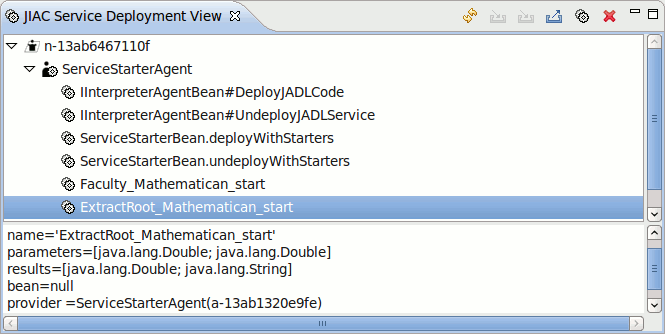
\includegraphics[width=.5\textwidth]{figures/features/deployment-view.png}
	\caption{The JIAC Service Deployment View.}
	\label{fig:deployView}
\end{figure}

While there are still some restrictions, e.g. service invocation from the
Deployment View currently works only for services with basic input and output
types (numbers, strings, etc.), these features are extremely helpful for developing
or composing new JIAC services -- both using the VSDT or the basic JADL source
code editor.


%%%%%%%%%%%%%%%%%%%%%%%%%%%%%%%%%%%%%%%%%%%%%%%%%%%%%%%%%%%%%%%%%%%%%%%%%%%%%%%%
%%  JIAC Fileserver View                                                      %%
%%%%%%%%%%%%%%%%%%%%%%%%%%%%%%%%%%%%%%%%%%%%%%%%%%%%%%%%%%%%%%%%%%%%%%%%%%%%%%%%

\section{JIAC File Server View}

As its name suggests, the JIAC File Server View is a client to the JIAC File Server,
a simple file server implemented using the JIAC frameworks and providing different
file operations as actions. The view provides buttons for listing, adding and removing
files (see Figure~\ref{fig:fileserverView}), and for copying the URL of a hosted file
to the clipboard. Files on the server can be opened directly into the Eclipse editor
and, after being edited, uploaded back to the server directly from the editor.

\begin{figure}[ht]
	\centering
	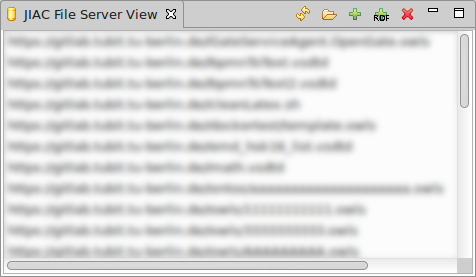
\includegraphics[width=.55\textwidth]{figures/features/fileserverview.png}
	\caption{The JIAC File Server View.}
	\label{fig:fileserverView}
\end{figure}

There exist different implementations of the JIAC fileserver, e.g. for hosting files
directly on the computer the node is running on, or for connecting to and hosting
the files on a Git repository. Further, the specialized OWL-S File Server will
automatically update the URIs internal to any OWL or OWL-S files uploaded to the
file server to their new location. This, too, can be used with the JIAC File
Server View using the \emph{Add RDF file...} button.


%%%%%%%%%%%%%%%%%%%%%%%%%%%%%%%%%%%%%%%%%%%%%%%%%%%%%%%%%%%%%%%%%%%%%%%%%%%%%%%%
%%  Process Engine Bean View                                                  %%
%%%%%%%%%%%%%%%%%%%%%%%%%%%%%%%%%%%%%%%%%%%%%%%%%%%%%%%%%%%%%%%%%%%%%%%%%%%%%%%%

\section{Process Engine Bean View}

This view presents an interface to the JIAC Process Engine Bean, i.e. the JIAC-enabled
VSDT interpreter agent (see Section 3.4 in the JIAC manual~\cite{jiacManual}). Similar
to the Service Deployment View, this view lists all reachable VSDT interpreter agents
and provides actions for listing (refreshing), uploading, and removing process interpreter
runtimes for the currently opened business process (see Figure~\ref{fig:processengineView}).

\begin{figure}[ht]
	\centering
	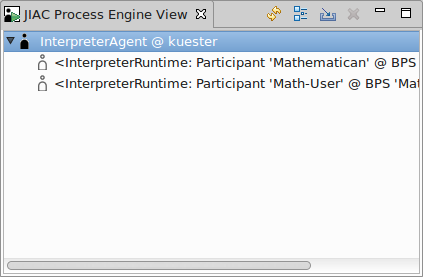
\includegraphics[width=.45\textwidth]{figures/features/processengineview.png}
	\caption{The JIAC Process Engine Bean View.}
	\label{fig:processengineView}
\end{figure}

This will take the VSDT process currently opened in the active editor window (if
any) and deploy it to the selected process engine bean. If the process provides
any actions (i.e. processes with a \emph{service} start event), then those can
again be found and invoked in the Service Deployment View described above, making
for a good prototyping- and testing-environment for developing composite processes.
For more control and runtime monitoring, you can use JIAC's Interpreter UI and
Introspection View~\cite[Sections 3.4 and 3.5]{jiacManual}.
